Рассмотрим более подробно выбранные алгоритмы сортировки. Для упрощения задачи будем сортировать последовательность по неубыванию. 
\section{Сортировка пузырьком}
\qquadОсуществляется проход по массиву от начала до конца, в процессе меняя местами неотсортированные соседние элементы.

В результате первого прохода на последнем месте окажется максимальный элемент. Далее снова делается проход по неотсортированной части массива (от первого до предпоследнего) и так же меняются неупорядоченные соседние элементы. Таким образом, на предпоследнее место будет помещён второй по величине элемент.

Действия повторяются до тех пор, пока не обработается вся неотсортированная часть. \\

\textbf{Схема} алгоритма представлена на Рис.\ref{fig1:image}.
\begin{figure}[h]
	\begin{center}
		{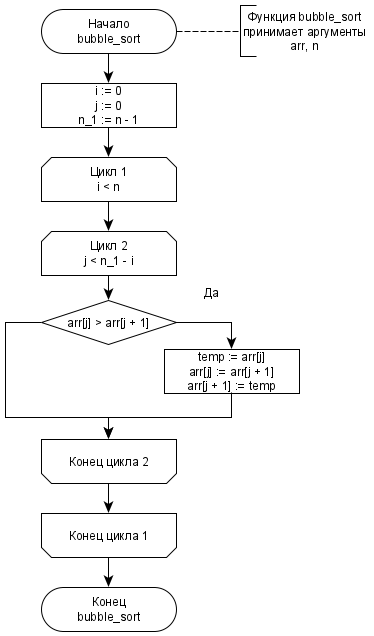
\includegraphics[scale = 0.519]{schemes/bubble}}
		\caption{Сортировка пузырьком}
		\label{fig1:image}
	\end{center}
\end{figure}

\section{Сортировка вставками}
\qquadВ этом алгоритме рассматриваемый массив условно делится на две части: отсортированная и нет. 

В начале работы отсортированной частью считается нулевой элемент. Далее берётся каждый следующий и сравнивается с уже отсортированной частью. Находится подходящая для текущего элемента позиция в ней, осуществляется сдвиг уже отсортированных элементов, но больших по величине, чем рассматриваемый. И затем рассматриваемый элемент помещается на найденную позицию.

И так до тех пор, пока не просмотрится вся неотсортированная часть.\\ 

\textbf{Схема} алгоритма представлена на Рис.\ref{fig2:image}.
\begin{figure}[pt!]
	\begin{center}
		{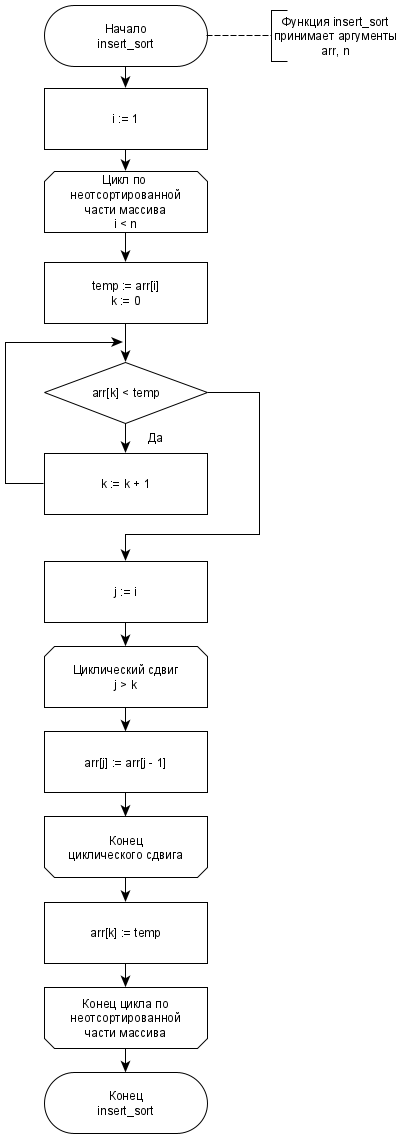
\includegraphics[scale = 0.57]{schemes/insert}}
		\caption{Сортировка вставками}
		\label{fig2:image}
	\end{center}
\end{figure}
\newpage

\section{Поразрядная сортировка}
\qquadПроизводится сортировка массива целых положительных чисел, а также чисел, которые можно преобразовать в неотрицательные, путём увеличения всех элементов на величину, равную модулю минимального элемента.\\

Перед началом работы алгоритма находится максимальное количество разрядов $k$ среди рассматриваемых чисел.\\

Далее сравнение производится поразрядно: сначала рассматриваются значения одного крайнего разряда, и формируются группы элементов по результатам этого сравнения, затем сравниваются значения следующего соседнего разряда, и происходит переупорядочивание элементов по результатам текущего сравнения (с сохранением относительного порядка, который был достигнут ранее). Сравнения продолжаются до тех пор, пока не обработается $k$ый разряд.\\

\textbf{Схема} алгоритма представлена на Рис.\ref{fig3:image} и \ref{fig4:image}.
\begin{figure}[pt!]
	\begin{center}
		{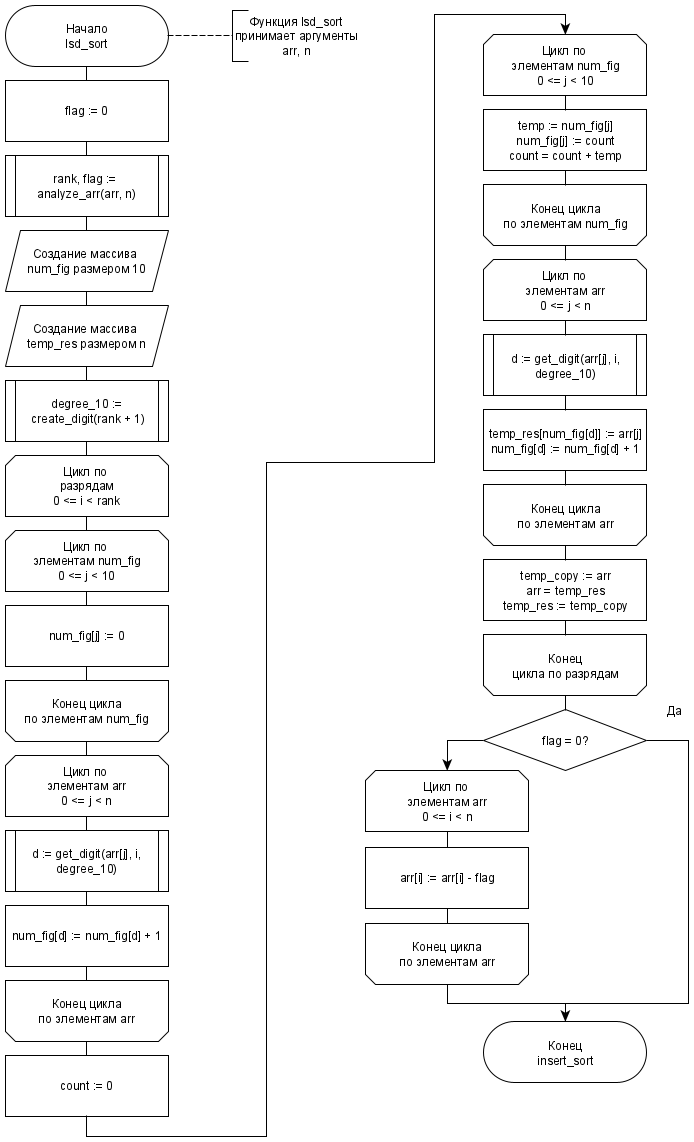
\includegraphics[scale = 0.55]{schemes/lsd_1}}
		\caption{Поразрядная сортировка (часть 1)}
		\label{fig3:image}
	\end{center}
\end{figure}

\begin{figure}[pt!]
	\begin{center}
		{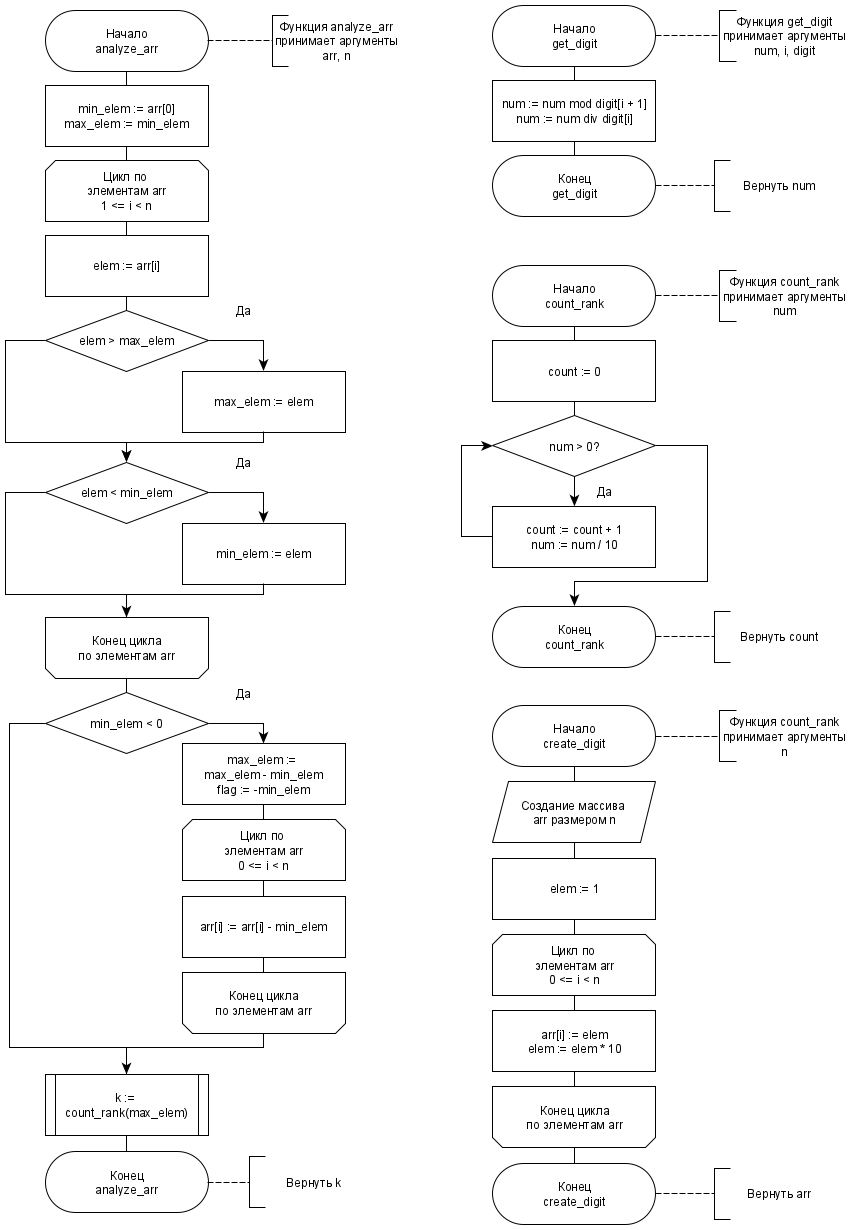
\includegraphics[scale = 0.53]{schemes/lsd_2}}
		\caption{Поразрядная сортировка (часть 2)}
		\label{fig4:image}
	\end{center}
\end{figure}

\newpage

\section{Требования к ПО}
\qquadДля корректной работы алгоритмов и проведения тестов необходимо выполнить следующее.
\begin{itemize}
	\item Обеспечить возможность ввода массива через консоль и выбора алгоритма сортировки.
	\item В случае ввода некорректных данных вывести соответствующее сообщение. Программа не должна аварийно завершаться.
	\item Программа должна отсортировать массив и вывести результат на экран.
	\item Реализовать функцию замера процессорного времени, которое выбранный метод затрачивает на вычисление результатов. Вывести результаты замеров на экран.
\end{itemize}

\section{Заготовки тестов}
\qquadПри проверке на корректность работы реализованных функций необходимо провести следующие тесты:
\begin{itemize}
	\item массив размером в один элемент;
	\item простой массив ненулевой длины;
	\item упорядоченный по невозрастанию массив;
	\item упорядоченный по неубыванию массив;
	\item массив, состоящий из одинаковых элементов.
\end{itemize}

\section*{Вывод}
\addcontentsline{toc}{section}{Вывод}
\qquadВ этом разделе детально разобраны основные шаги выбранных алгоритмов, построены схемы их работы. Также описаны требования к программному обеспечению и приведены заготовки тестов.